\pdfbookmark{Общая характеристика работы}{characteristic}             % Закладка pdf
\section*{Общая характеристика работы}

\newcommand{\actuality}{\pdfbookmark[1]{Актуальность}{actuality}\underline{\textbf{\actualityTXT}}}
\newcommand{\progress}{\pdfbookmark[1]{Разработанность темы}{progress}\underline{\textbf{\progressTXT}}}
\newcommand{\aim}{\pdfbookmark[1]{Цели}{aim}\underline{{\textbf\aimTXT}}}
\newcommand{\object}{\pdfbookmark[1]{Объект исследования}{object}\underline{\textbf{\objectTXT}}}
\newcommand{\subject}{\pdfbookmark[1]{Предмет исследования}{subject}\underline{\textbf{\subjectTXT}}}
\newcommand{\tasks}{\pdfbookmark[1]{Задачи}{tasks}\underline{\textbf{\tasksTXT}}}
\newcommand{\aimtasks}{\pdfbookmark[1]{Цели и задачи}{aimtasks}\aimtasksTXT}
\newcommand{\novelty}{\pdfbookmark[1]{Научная новизна}{novelty}\underline{\textbf{\noveltyTXT}}}
\newcommand{\influence}{\pdfbookmark[1]{Практическая значимость}{influence}\underline{\textbf{\influenceTXT}}}
\newcommand{\methods}{\pdfbookmark[1]{Методология и методы исследования}{methods}\underline{\textbf{\methodsTXT}}}
\newcommand{\defpositions}{\pdfbookmark[1]{Положения, выносимые на защиту}{defpositions}\underline{\textbf{\defpositionsTXT}}}
\newcommand{\reliability}{\pdfbookmark[1]{Достоверность}{reliability}\underline{\textbf{\reliabilityTXT}}}
\newcommand{\probation}{\pdfbookmark[1]{Апробация}{probation}\underline{\textbf{\probationTXT}}}
\newcommand{\contribution}{\pdfbookmark[1]{Личный вклад}{contribution}\underline{\textbf{\contributionTXT}}}
\newcommand{\publications}{\pdfbookmark[1]{Публикации}{publications}\underline{\textbf{\publicationsTXT}}}

    \nocite{костенко2020исследование}%
    \nocite{костенко2020методы}%
    \nocite{костенко2017оценка}%
    \nocite{костенко2019задача}%
    %
    %% authorscopus
    \nocite{kostenko2021comparative}%
    \nocite{tolstonogov2017auv}
    %
    %% authorconf
    \nocite{костенко2020анализ}%
    \nocite{костенко2019разработка}%
    \nocite{костенко2019особенности}%
    \nocite{костенко2017разработка}%

{\actuality}
Задача распределения управляющих воздействий (control allocation) возникает естественным образом для избыточного (over-actuated) ДРК ПА, то есть такого ДРК в котором ИМ (рули управления, основные и подруливающие движители) больше чем количество доступных для управления степеней свободы. Использование ДРК такого типа широко распространено по следующим причинам:
\begin{itemize}
    \item в виду того, что подводные операции сопряжены с высокой степенью риска, избыточность необходима для реализации функций резервирования систем управления движением подводного аппарата;
    \item в силу гидродинамических особенностей функционирования при различных режимах движения (позиционный, крейсерский) часть исполнительных механизмов ДРК будет работать лучше или хуже; в соответствии с этим, при разработке многоцелевых подводных аппаратов необходимо использовать избыточные комплекты ИМ \cite{valasek2002design}.
    \item избыточная конфигурация ДРК при энергетически оптимальном распределении управляющего воздействия позволяет сократить затраты энергии на 20-25\% по сравнению с эквивалентной неизбыточной конфигурацией \cite{бриллиантов2005разработка}.
\end{itemize}

Решение задачи распределения управляющих воздействий ДРК позволяет оптимизировать энергетические затраты на движение ПА, обеспечить отказоустойчивость системы управления, и уменьшить механический износ ИМ в условиях накладываемых на них ограничений \cite{enns1998control}.
Исторически первой эта задача возникла в двух областях: для систем управления многостепенными манипуляторами \cite{craig2009introduction} и самолётами \cite{bordignon1996constrained}. 
Основной целью тогда было создание систем аккомодации, то есть формирования такой системы управления движением, которая была бы устойчива к выходу из строя отдельных исполнительных механизмов.

В общем случае задача распределения управляющих воздействий для случая избыточных систем управления ведет к задаче численной оптимизации с линейными ограничениями, решение которой сложно реализовать для высокочастотных управляющих контуров в условиях операционных систем реального времени.

В настоящее время имеется достаточное количество обзорных статей в иностранной научной литературе, посвященных задаче распределения управляющих воздействий, включая как отдельные приложения – суда, подводные аппараты  \cite{fossen2006survey}, летательные средства \cite{oppenheimer2006control}, так и междисциплинарные \cite{10.1016/j.automatica.2013.01.035}.
В отечественной литературе такая постановка задачи обычно не выделяется в отдельный класс \cite{филаретов2016особенности} и, например, задача аккомодации к отказам исполнительных механизмов решается в рамках управления объектом целиком  \cite{мартынова2020подход, зыбин2014аналитическое}.
Впрочем, упоминание задачи распределения управляющих воздействий можно найти в отдельных статьях \cite{амбросовский2013распределение, воловодов2003распределение, амбросовский2014алгоритмы} и главах диссертаций \cite{власов2016адаптивное}.

% \ifsynopsis
% Этот абзац появляется только в~автореферате.
% Для формирования блоков, которые будут обрабатываться только в~автореферате,
% заведена проверка условия \verb!\!\verb!ifsynopsis!.
% Значение условия задаётся в~основном файле документа (\verb!synopsis.tex! для
% автореферата).
% \else
% Этот абзац появляется только в~диссертации.
% Через проверку условия \verb!\!\verb!ifsynopsis!, задаваемого в~основном файле
% документа (\verb!dissertation.tex! для диссертации), можно сделать новую
% команду, обеспечивающую появление цитаты в~диссертации, но~не~в~автореферате.
% \fi

% {\progress}
% Этот раздел должен быть отдельным структурным элементом по
% ГОСТ, но он, как правило, включается в описание актуальности
% темы. Нужен он отдельным структурынм элемементом или нет ---
% смотрите другие диссертации вашего совета, скорее всего не нужен.

{\aim} диссертационной работы является разработка методов энергоэффективного и отказоустойчивого управления избыточным движительно-рулевым комплексом подводного аппарата с учётом динамики исполнительных механизмов и их гидродинамических особенностей.

Для~достижения поставленной цели необходимо было решить следующие {\tasks}:
\begin{enumerate}[beginpenalty=10000] % https://tex.stackexchange.com/a/476052/104425
  \item изучить модели описания исполнительных механизмов (маршевые движители, подруливающие движители, рули управления) ДРК подводного аппарата учитывающие особенности их поведения в набегающем потоке;
  \item разработать метод формального описания, анализа и реконфигурации в режиме реального времени ДРК оснащенного произвольным набором исполнительных механизмов;
  \item разработать и реализовать дублирующий метод определения скорости набегающего потока по параметрам работы электроприводов маршевых движителей;
  \item разработать и реализовать энергетически оптимальный отказоустойчивый метод распределения управляющих воздействий для АНПА устойчивый к неполному знанию скорости набегающего потока;
  \item разработать и реализовать метод плавного перераспределения управляющего воздействия при переходах между различными типами движения;
  \item провести проверку эффективности разработанного метода распределения управляющих воздействий на базе модельных экспериментов.
\end{enumerate}

{\novelty}
\begin{enumerate}[beginpenalty=10000] % https://tex.stackexchange.com/a/476052/104425
  \item разработан метод определения скорости движения подводного аппарата относительно воды в установившемся режиме по изменению параметров работы маршевых движителей;
  \item разработан метод формирования глобальных границ и коэффициентов решения задачи оптимального распределения управляющих воздействий ДРК адаптивный к скорости набегающего потока и оценки его достоверности;
  \item разработан метод перераспределения управляющих воздействий при смене типа движения многофункционального АНПА.
\end{enumerate}

{\influence} \ldots

{\methods} В диссертационной работе использовались методы теории управления, линейной и нелинейной оптимизации; методы математического и имитационного моделирования, современные средства разработки программных комплексов и моделирования.

{\defpositions}
\begin{enumerate}[beginpenalty=10000] % https://tex.stackexchange.com/a/476052/104425
  \item Предложен метод формального описания и анализа ДРК подводного аппарата, который отличается тем, что каждый движитель 

  с произвольным количеством и типом используемых исполнительных механизмов и его программная реализация;
  \item метод оценки скорости движения подводного аппарата относительно воды в установившемся режиме по изменению параметров работы его маршевых движителей;
  \item метод энергоэффективного и отказоустойчивого распределения управляющих воздействий на ДРК подводного аппарата адаптивный к скорости набегающего потока и оценки его достоверности;
  \item программная реализация метода перераспределения управляющих воздействий при смене типа движения многофункционального АНПА.
\end{enumerate}

{\reliability} Достоверность полученных выводов определяется корректным применением методов математического моделирования сложных систем и обработки экспериментальных данных. Обоснованность полученных методов и алгоритмов основывается на сопоставлении полученных результатов с результатами, полученными другими известными методами и алгоритмами.

{\probation}
Основные результаты диссертации
докладывались и обсуждались на следующих конференциях:
\begin{enumerate}
    \item ``Управление в морских и аэрокосмических системах (УМАС-2016)'' (Санкт-Петербург, 04–06 октября 2016 года);
    \item Всероссийская научно-техническая конференция ``Технические проблемы освоения мирового океана'' (г. Владивосток, 2017);
    \item ``International Symposium on Underwater Technology, UT'' (Haeundae, Busan, 21–24 февраля 2017 года);
    \item ``2018 OCEANS - MTS/IEEE Kobe Techno-Oceans, OCEANS - Kobe 2018'' (Kobe, 28–31 мая 2018 года);
    \item Всероссийская научно-техническая конференция ``Технические проблемы освоения мирового океана'' (г. Владивосток, 30 сентября – 3 октября 2019 г.);
    \item ``2019 IEEE International Underwater Technology Symposium, UT 2019'' (Kaohsiung, 16–19 апреля 2019 года);
    \item Международная конференция по промышленному инжинирингу и современным технологиям ``FarEastCon-2019'' (г. Владивосток, 1-4 сентября 2019 года);
    \item Международная конференция по промышленному инжинирингу и современным технологиям ``FarEastCon-2020'' (г. Владивосток, 5-8 октября 2019 года);
    \item ``Global Oceans 2020: Singapore - U.S. Gulf Coast'' (5-14 октября 2020 года);
    \item 
\end{enumerate}

{\contribution} Автор принимал участие в постановке цели и задач по теме исследования, разработал методы и алгоритмы, предложенные в данной работе, обработал и проанализировал экспериментальные данные, участвовал в обсуждении полученных результатов, подготовке научных статей, материалов конференций, участвовал на конференциях и семинарах.

\ifnumequal{\value{bibliosel}}{0}
{%%% Встроенная реализация с загрузкой файла через движок bibtex8. (При желании, внутри можно использовать обычные ссылки, наподобие `\cite{vakbib1,vakbib2}`).
    {\publications} Основные результаты по теме диссертации изложены
    в~XX~печатных изданиях,
    X из которых изданы в журналах, рекомендованных ВАК,
    X "--- в тезисах докладов.
}%
{%%% Реализация пакетом biblatex через движок biber
    \begin{refsection}[bl-author, bl-registered]
        % Это refsection=1.
        % Процитированные здесь работы:
        %  * подсчитываются, для автоматического составления фразы "Основные результаты ..."
        %  * попадают в авторскую библиографию, при usefootcite==0 и стиле `\insertbiblioauthor` или `\insertbiblioauthorgrouped`
        %  * нумеруются там в зависимости от порядка команд `\printbibliography` в этом разделе.
        %  * при использовании `\insertbiblioauthorgrouped`, порядок команд `\printbibliography` в нём должен быть тем же (см. biblio/biblatex.tex)
        %
        % Невидимый библиографический список для подсчёта количества публикаций:
        \printbibliography[heading=nobibheading, section=1, env=countauthorvak,          keyword=biblioauthorvak]%
        \printbibliography[heading=nobibheading, section=1, env=countauthorwos,          keyword=biblioauthorwos]%
        \printbibliography[heading=nobibheading, section=1, env=countauthorscopus,       keyword=biblioauthorscopus]%
        \printbibliography[heading=nobibheading, section=1, env=countauthorconf,         keyword=biblioauthorconf]%
        \printbibliography[heading=nobibheading, section=1, env=countauthorother,        keyword=biblioauthorother]%
        \printbibliography[heading=nobibheading, section=1, env=countregistered,         keyword=biblioregistered]%
        \printbibliography[heading=nobibheading, section=1, env=countauthorpatent,       keyword=biblioauthorpatent]%
        \printbibliography[heading=nobibheading, section=1, env=countauthorprogram,      keyword=biblioauthorprogram]%
        \printbibliography[heading=nobibheading, section=1, env=countauthor,             keyword=biblioauthor]%
        \printbibliography[heading=nobibheading, section=1, env=countauthorvakscopuswos, filter=vakscopuswos]%
        \printbibliography[heading=nobibheading, section=1, env=countauthorscopuswos,    filter=scopuswos]%
        %
        \nocite{*}%
        %
        {\publications} Основные результаты по теме диссертации изложены в~\arabic{citeauthor}~печатных изданиях,
        \arabic{citeauthorvak} из которых изданы в журналах, рекомендованных ВАК\sloppy%
        \ifnum \value{citeauthorscopuswos}>0%
            , \arabic{citeauthorscopuswos} "--- в~периодических научных журналах, индексируемых Web of~Science и Scopus\sloppy%
        \fi%
        \ifnum \value{citeauthorconf}>0%
            , \arabic{citeauthorconf} "--- в~тезисах докладов.
        \else%
            .
        \fi%
        \ifnum \value{citeregistered}=1%
            \ifnum \value{citeauthorpatent}=1%
                Зарегистрирован \arabic{citeauthorpatent} патент.
            \fi%
            \ifnum \value{citeauthorprogram}=1%
                Зарегистрирована \arabic{citeauthorprogram} программа для ЭВМ.
            \fi%
        \fi%
        \ifnum \value{citeregistered}>1%
            Зарегистрированы\ %
            \ifnum \value{citeauthorpatent}>0%
            \formbytotal{citeauthorpatent}{патент}{}{а}{}\sloppy%
            \ifnum \value{citeauthorprogram}=0 . \else \ и~\fi%
            \fi%
            \ifnum \value{citeauthorprogram}>0%
            \formbytotal{citeauthorprogram}{программ}{а}{ы}{} для ЭВМ.
            \fi%
        \fi%
        % К публикациям, в которых излагаются основные научные результаты диссертации на соискание учёной
        % степени, в рецензируемых изданиях приравниваются патенты на изобретения, патенты (свидетельства) на
        % полезную модель, патенты на промышленный образец, патенты на селекционные достижения, свидетельства
        % на программу для электронных вычислительных машин, базу данных, топологию интегральных микросхем,
        % зарегистрированные в установленном порядке.(в ред. Постановления Правительства РФ от 21.04.2016 N 335)
    \end{refsection}%
    \begin{refsection}[bl-author, bl-registered]
        % Это refsection=2.
        % Процитированные здесь работы:
        %  * попадают в авторскую библиографию, при usefootcite==0 и стиле `\insertbiblioauthorimportant`.
        %  * ни на что не влияют в противном случае
        \nocite{vakbib2}%vak
        \nocite{patbib1}%patent
        \nocite{progbib1}%program
        \nocite{bib1}%other
        \nocite{confbib1}%conf
    \end{refsection}%
        %
        % Всё, что вне этих двух refsection, это refsection=0,
        %  * для диссертации - это нормальные ссылки, попадающие в обычную библиографию
        %  * для автореферата:
        %     * при usefootcite==0, ссылка корректно сработает только для источника из `external.bib`. Для своих работ --- напечатает "[0]" (и даже Warning не вылезет).
        %     * при usefootcite==1, ссылка сработает нормально. В авторской библиографии будут только процитированные в refsection=0 работы.
}

% При использовании пакета \verb!biblatex! будут подсчитаны все работы, добавленные
% в файл \verb!biblio/author.bib!. Для правильного подсчёта работ в~различных
% системах цитирования требуется использовать поля:
% \begin{itemize}
%         \item \texttt{authorvak} если публикация индексирована ВАК,
%         \item \texttt{authorscopus} если публикация индексирована Scopus,
%         \item \texttt{authorwos} если публикация индексирована Web of Science,
%         \item \texttt{authorconf} для докладов конференций,
%         \item \texttt{authorpatent} для патентов,
%         \item \texttt{authorprogram} для зарегистрированных программ для ЭВМ,
%         \item \texttt{authorother} для других публикаций.
% \end{itemize}
% Для подсчёта используются счётчики:
% \begin{itemize}
%         \item \texttt{citeauthorvak} для работ, индексируемых ВАК,
%         \item \texttt{citeauthorscopus} для работ, индексируемых Scopus,
%         \item \texttt{citeauthorwos} для работ, индексируемых Web of Science,
%         \item \texttt{citeauthorvakscopuswos} для работ, индексируемых одной из трёх баз,
%         \item \texttt{citeauthorscopuswos} для работ, индексируемых Scopus или Web of~Science,
%         \item \texttt{citeauthorconf} для докладов на конференциях,
%         \item \texttt{citeauthorother} для остальных работ,
%         \item \texttt{citeauthorpatent} для патентов,
%         \item \texttt{citeauthorprogram} для зарегистрированных программ для ЭВМ,
%         \item \texttt{citeauthor} для суммарного количества работ.
% \end{itemize}
% % Счётчик \texttt{citeexternal} используется для подсчёта процитированных публикаций;
% % \texttt{citeregistered} "--- для подсчёта суммарного количества патентов и программ для ЭВМ.

% Для добавления в список публикаций автора работ, которые не были процитированы в
% автореферате, требуется их~перечислить с использованием команды \verb!\nocite! в
% \verb!Synopsis/content.tex!.
 % Характеристика работы по структуре во введении и в автореферате не отличается (ГОСТ Р 7.0.11, пункты 5.3.1 и 9.2.1), потому её загружаем из одного и того же внешнего файла, предварительно задав форму выделения некоторым параметрам

%Диссертационная работа была выполнена при поддержке грантов \dots

%\underline{\textbf{Объем и структура работы.}} Диссертация состоит из~введения,
%четырех глав, заключения и~приложения. Полный объем диссертации
%\textbf{ХХХ}~страниц текста с~\textbf{ХХ}~рисунками и~5~таблицами. Список
%литературы содержит \textbf{ХХX}~наименование.

\pdfbookmark{Содержание работы}{description}                          % Закладка pdf
\section*{Содержание работы}

Во \underline{\textbf{введении}} обосновывается актуальность
исследований, проводимых в~рамках данной научно-квалификационной работы,
приводится обзор научной литературы по~изучаемой проблеме,
формулируется цель, ставятся задачи работы, излагается научная новизна
и практическая значимость представляемой работы.


\underline{\textbf{Первая глава}} посвящена обзору современных методов и подходов к решению задачи энергоэффективного управления ДРК.

Отмечено, что хоть тема достаточно проработана, но в работах почти никак не фигурируют гидродинамические особенности работы исполнительных механизмов в набегающем потоке и уменьшение их результирующей силы.

Во \underline{\textbf{второй главе}} приведены математические модели исполнительных механизмов (маршевые движители, подруливающие движители, рули управления) ДРК ПА учитывающие особенности их работы в набегающем потоке.
Показано, что эффективность работы ИМ существенным образом зависят от скорости набегающего потока. 
Приведены результаты численного моделирования работы ИМ.

Отдельное внимание в главе уделено поведению подруливающих движителей в набегающем потоке.
Показано что эффективный упор создаваемый подруливающими движителями падает экспоненциально и для представленных в главе параметров подруливающего ИМ падает до около нулевых значений при скорости набегающего потока 1.5 м/с.

В работах на которые автор ссылается показано, что падение эффективности подруливающего движителя связано не с уменьшением эффективности самого устройства, а с взаимодействием пропульсивной струи, которую создает подруливающий движитель, с набегающим на ПА потоком.

Работа подруливающего движителя ПА при отсутствии поперечного потока полностью эквивалентна модели маршевого движителя, т.е. на аппарат действует определенная сила (упор) приложенная к точке крепления движителя за счет формирования пропульсивной струи ПА.
Но в случае, когда ПА движется с продольной скоростью $u$, то пропульсивная струя формируемая подруливающим движителем формирует гидродинамическую тень (на рисунке закрашена серым цветом) на корпусе ПА в области за подруливающей шахтой (рисунок 1).
За счет этого формируется разность давлений между различными областями ПА, которая, в свою очередь, формирует силу $T_S$ обратную по направлению к силе создаваемой подруливающим движителем $T_T$.

\begin{figure}[ht]
    \centering
    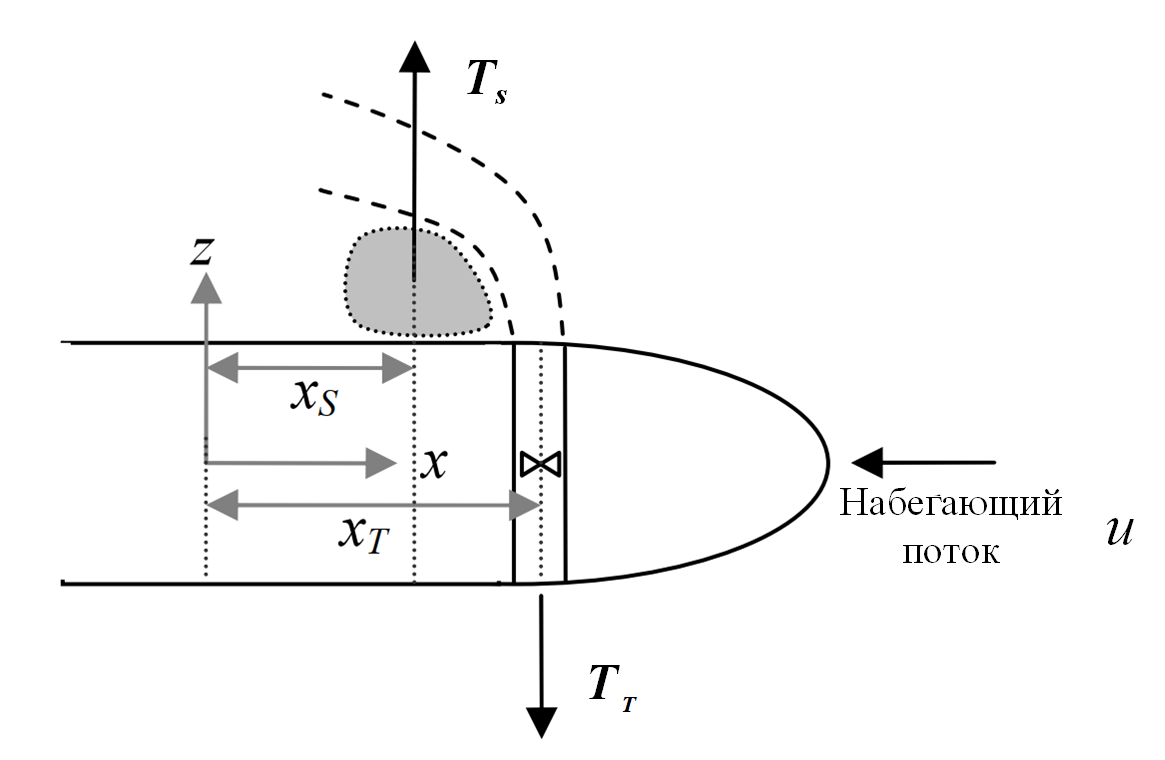
\includegraphics[width=0.6\linewidth]{modelling/Моделирование - подруливающий движитель силы.png}
    \caption*{Рис 1. -- Особенности поведения подруливающего движителя в набегающем потоке.}
    \label{fig:modelling-tunnel}
\end{figure}

При низких и средних скоростях продольного движения ПА, когда формируемая подруливающим движителем скорость пропульсивной струи существенно выше скорости АНПА наклон струи незначителен, гидродинамическая тень мала и соответственно мала и сила создаваемая разностью давлений на корпус ПА.
При высоких скоростях движения ПА, когда скорость набегаемого на АПНА потока сопоставима или выше по скорости чем скорость создаваемой подруливающим движителем пропульсивной струи, её наклон существенно выше, как и создаваемая гидродинамическая тень и общая эффективность подруливающего движителя падает значительно.

В работе \cite{palmer2009analysis} предложено силу формируемую разностью давлений представлять следующим образом:
\begin{equation}
    \label{eq:thrust_tunnel}
    T_S = T_T (1 - \exp \left[ -c \left( \frac{u}{u_j} \right)^2 \right])
\end{equation}
\noindent где
\begin{itemize}
    \item $T_S$ -- сила действующая на аппарат в связи с разностью давлений;
    \item $T_T$ -- упор создаваемый подруливающим движителем;
    \item $u$ -- скорость набегающего потока;
    \item $u_j$ -- скорость пропульстивной струи;
    \item $c$ -- коэффициент подавления упора.
\end{itemize}

В свою очередь скорость пропульсивной струи, создаваемой работой подруливающего движителя, может быть определена следующим уравнением:
\begin{equation}
    \label{eq:jetflow_speed}
    u_j = \sqrt{\frac{T_T(v=0)}{\rho A}}
\end{equation}
\noindent где $T_T(v=0)$ -- упор создаваемый подруливающим движителем в отсутствии набегающего потока, $\rho$ -- плотность воды, $A=\pi R^2$, где $R$ -- радиус гребного винта подруливающего движителя.

В главе так же представлены результаты численного моделирования влияния набегающего потока на величину сил и моментов создаваемых различными типами исполнительных механизмов (рисунок 2).

\begin{figure}[ht]
    \centerfloat{
        \hfill
        \subcaptionbox{Подруливающий движитель}{%
            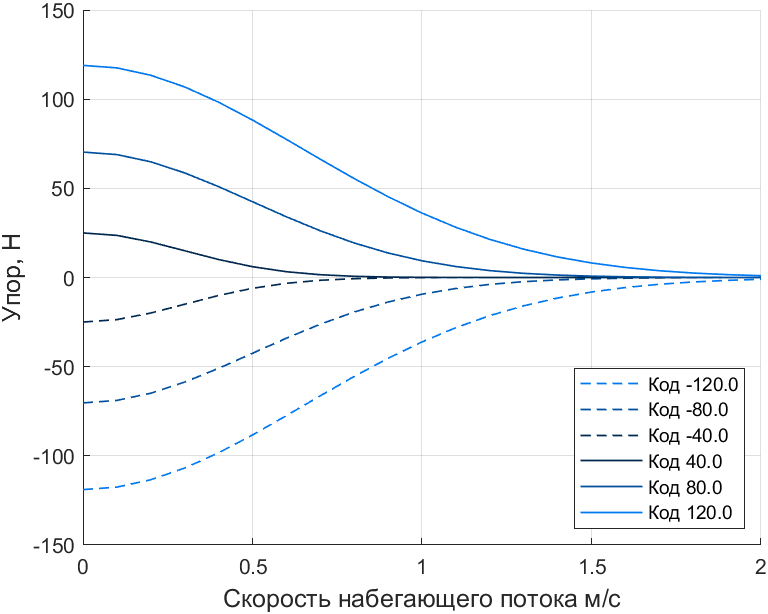
\includegraphics[width=0.5\linewidth]{modelling/Моделирование - подруливающий движитель скорость.png}}
        \hfill
        \subcaptionbox{Маршевый движитель}{%
            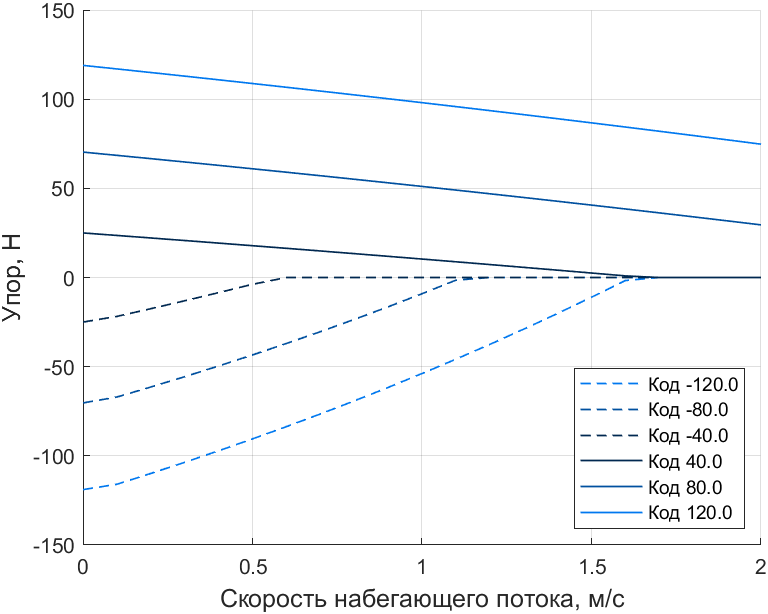
\includegraphics[width=0.5\linewidth]{modelling/Моделирование - маршевый движитель скорость.png}}
        \hfill
    }
    \caption*{Рис. 2 -- Численное моделирование установившегося эффективного упора создаваемого ИМ при различных скоростях набегающего потока.}\label{fig:latex}
\end{figure}


Содержимое \underline{\textbf{третьей главы}} посвящено разработке метода оценки скорости набегающего потока в установившемся режиме движения АНПА по изменению параметров работы движителей маршевой группы.
Оценка скорости набегающего потока была получена на основе линеаризации в ограниченных пределеах коэффициентов упора и момента гребного винта $K_T (J_0), K_Q (J_0)$:
\begin{gather}
    K_T = K_T^{bp} - \alpha_1 J_0 \notag \\
    K_Q = K_Q^{bp} - \beta_1 J_0 \label{eq:torque_linear}
\end{gather}
\noindent где $K_T^{bp}, K_Q^{bp}$ -- коэффициенты упора и момента гребного винта полученные в результате швартовых испытаний движителя, а в свою очередь, а $J_0$ -- относительная поступь определяемая следующим образом:
\begin{equation*}
    J_0 = \frac{v}{nD}
\end{equation*}
\noindent где $v$ -- скорость набегающего потока, $n$ -- скорость вращения вала, $D$ -- диаметр винта.

Из этих уравнений и на основе математической модели электрического привода движителя можно оценить скорость набегающего потока следующим образом:
\begin{equation}
    \label{eq:velocity_final}
    v = \frac{1}{\beta_1} \left( K_Q^{bp} n D - K_m\frac{I}{\rho D^4|n|n} \right)
\end{equation}
\noindent где $K_m$ -- постоянная момента электропривода, а $I$ -- ток на его обмотках.

Была проведена верификация метода на обработке данных запусков АНПА ``ММТ-3000'' в заливе Патрокл.
После уточнения параметров ГВ на калибровочной части маршрута, расхождение оцениваемой скорости с эталонными показаниями доплеровского лага составило не более чем 0.18 м/с на переходных режимах и не более чем 0.1 м/с на установившихся режимах движения со среднеквадратичным отклонением $\sigma=0.17$ м/с (рисунок 3).

\begin{figure}[ht]
    \centering
    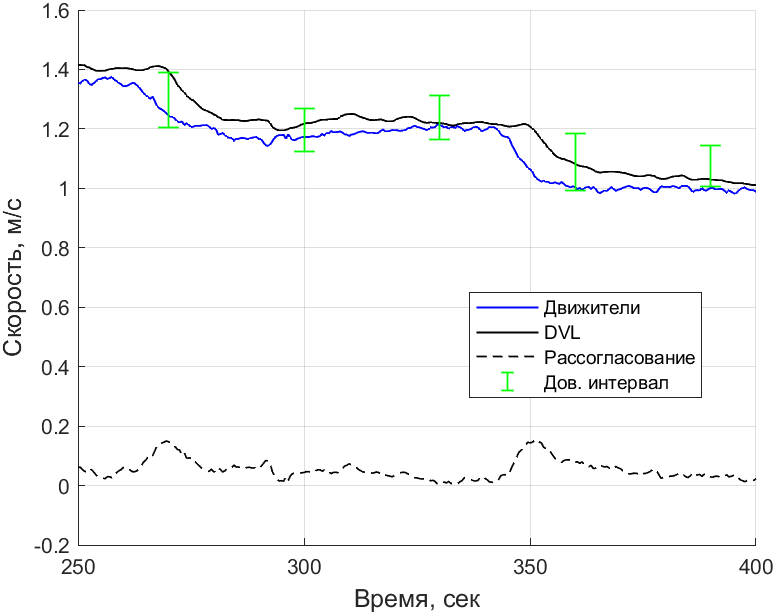
\includegraphics[width=0.6\linewidth]{velocity/ММТ3000 - тестирование b2.png}
    \caption* {Рис. 3 -- Cкорость продольного движения АНПА ``ММТ-3000'' по данным доплеровского лага и по оценке с движителей.}
    \label{fig:mmt3000_velocity_check}
\end{figure}

В \underline{\textbf{четвертой главе}} предложен новый алгоритм энергоэффективного управления ДРК подводного аппарата в условиях ограничений накладываемых на работу исполнительных механизмов, который учитывает особенности работы ИМ ДРК в набегающем потоке и способен адаптивно перераспределять управляющие воздействия при вариациях скорости.

Пусть функционал энергоэффективного управления ДРК $J(\vect{u})$, где $\vect{u}$ -- вектор команд управления ИМ ДРК, задаётся в квадратичной форме и имеет следующий вид \cite{burken2001two}:
\begin{equation}
    \label{eq:functional_weight}
    J = (1-\varepsilon)(BK(v)\vect{u} - \vect{\nu})^TQ_{\nu}(BK(v)\vect{u} - \vect{\nu}) + \varepsilon 
    \vect{u}^TQ_{u}\vect{u}
\end{equation}
\noindent где
\begin{itemize}
    \item $v$ -- скорость набегающего потока,
    \item $\vect{\nu}$ -- целевая команда управления АНПА,
    \item $\varepsilon$ -- весовой коэффициент отклика системы на управление, $0 < \varepsilon < 1$;
    \item $Q_{\nu}$ -- диагональная матрица положительно определенных весовых коэффициентов осей управления;
    \item $Q_{u}$ -- диагональная матрица положительно определенных весовых коэффициентов ИМ;
    \item $K(v)$ -- матрица коэффициентов поведения ИМ в потоке, детальное описание которой приведено в работе.
\end{itemize}

Для решения задачи поиска оптимального решения по заданному функционалу было использовано итерационное глобально-сходящееся решение следующего вида:
\begin{equation}
    \label{eq:Allocation/FixedMethod}
    \vect{u}_{n+1} = \text{sat}
    \left[
    (1-\varepsilon)\omega (BK(v))^TQ_{\nu}\nu - (\omega H - I) \vect{u}_{n}
    \right]
\end{equation}
\noindent где
\begin{itemize}
    \item $H=(1 - \varepsilon)(BK(v))^TQ_{\nu}B + \varepsilon Q_u$;
    \item $\omega = 1 / ||H||_2$, где $||\cdot||_2$ -- норма оператора в $L_2$;
    \item $I$ -- диагональная единичная матрица;
    \item $\vect{u}_{n+1}$ -- вектор управления ДРК на $n+1$ шаге итерационного расчёта.
\end{itemize}

Итеративный расчёт вектора $\vect{u}$ заканчивается при выполнении следующего неравенства:
\begin{equation*}
    \left| J(\vect{u}_{k+1}) - J(\vect{u}_{k}) \right| < J_{end}
\end{equation*}
\noindent где $J_{end}$ -- настраиваемый параметр, который зависит от дискретности управления исполнительными механизмами ДРК.

В случае если рассматривается задача не предусматривающая ограничений (т.е. $\mathspace{U} = \mathspace{R}$) или решение задачи оптимального управления укладывается в заданные ограничения, т.е. $\vect{u^*} \in \mathspace{U}$, то решение можно получить аналитически через частную производную от функционала $\frac{\partial J}{\partial u}$. Тогда вектор оптимального управления будет следующим:
\begin{equation*}
    \vect{u^*} = (1-\epsilon)\left[(1-\epsilon)(BK(v))^{-1}Q_{\nu}BK(v) + \epsilon Q_u\right](BK(v))^TQ_{\nu} \vect{\nu}_c
\end{equation*}

Общая структурная блок-схема работы алгоритма управления ДРК с учетом оценки скорости набегающего потока по математической модели маршевых движителей представлена на рисунке 4.

\begin{figure}[ht]
    \centering
    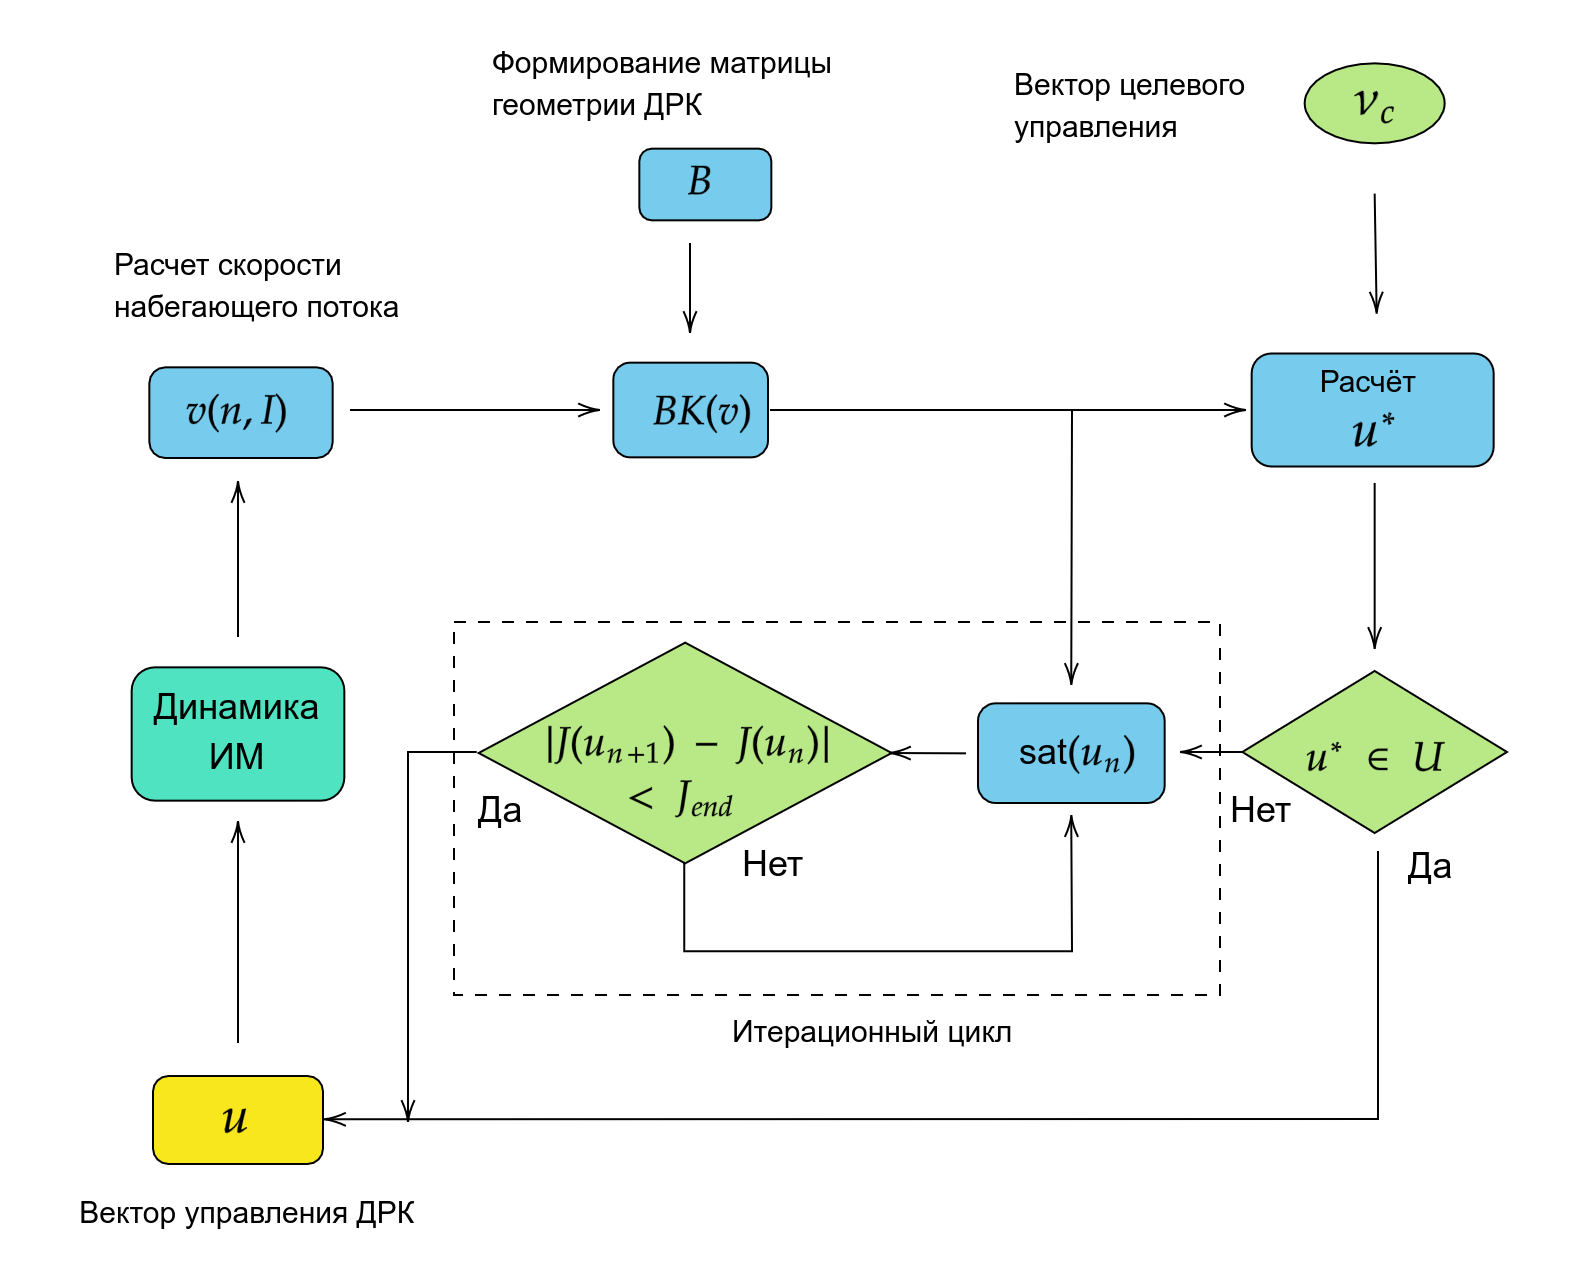
\includegraphics[width=0.8\linewidth]{allocation/Алгоритм - Блок-схема.png}
    \caption*{Рис. 4 -- Общая блок-схема реализации алгоритма адаптивного управления ДРК.}
    \label{fig:method_algorithm}
\end{figure}

В главе также проведён численный анализ эффективности представленного адаптивного метода управления ДРК на базе модели ДРК АНПА ``ММТ-300''\cite{борейко2019малогабаритный}.

Кроме этого, было проведено сравнение предлагаемого адаптивного метода управления ДРК при различных вариациях скорости набегающего потока относительно того, который реализован в СУ на АНПА ``ММТ-3000'', который разработан в ИПМТ ДВО РАН.

Результаты распределения упоров и формируемые при этом силы и моменты методом прямого управления ДРК с масштабированием реализованного в СУ АНПА ``ММТ-3000'' в диапазоне скоростей от 0 до 2.5 м/с представлены на рисунке 5.
Аналогичные данные для предлагаемого адаптивного метода управления ДРК представлены на рисунке 6.

\begin{figure}[ht]
    \centerfloat{
        \hfill
        \subcaptionbox{Команды ИМ}{%
            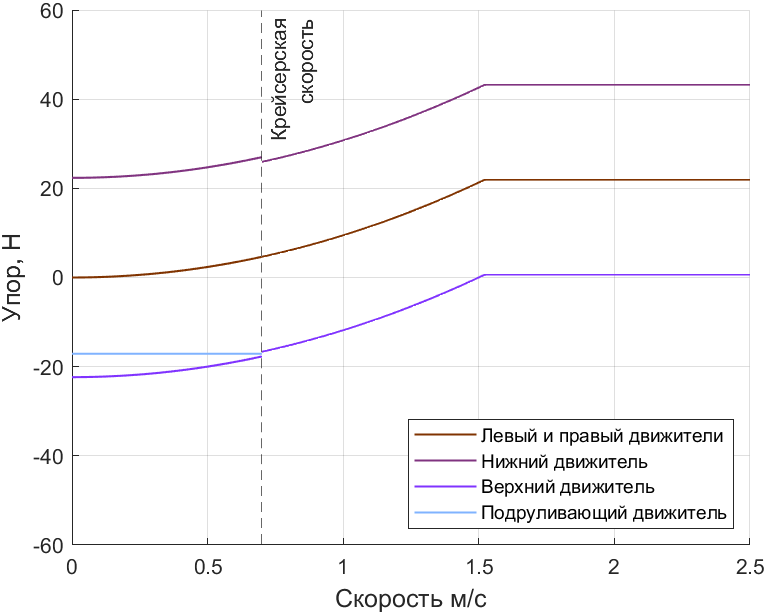
\includegraphics[width=0.5\linewidth]{allocation/Результат ММТ300 - Стандартный упоры.png}}
        \hfill
        \subcaptionbox{Сформированные силы и моменты}{%
            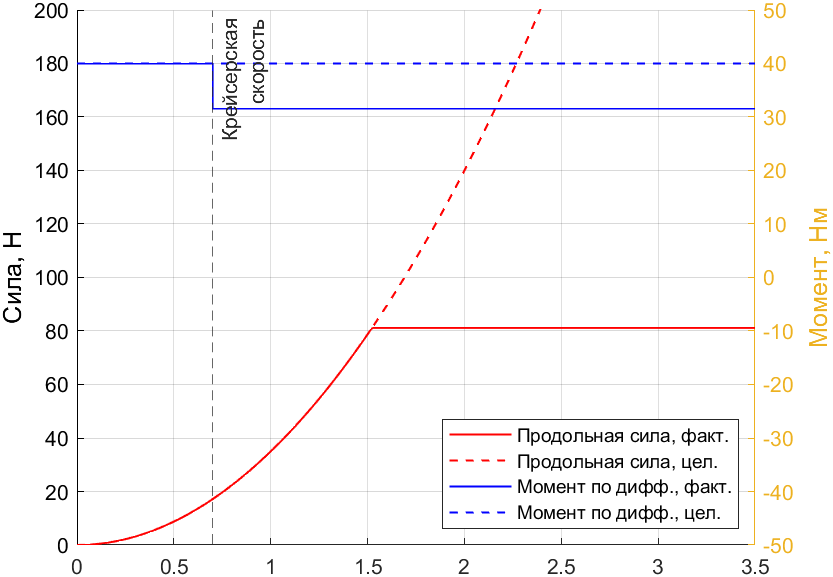
\includegraphics[width=0.5\linewidth]{allocation/Результат ММТ300 - Стандартный силы.png}}
        \hfill
    }
    \caption*{Рис. 5 -- Распределение упоров и сформированные при этом силы и моменты методом прямого управления ДРК с масштабированием.}\label{fig:latex}
\end{figure}

\begin{figure}[ht]
    \centerfloat{
        \hfill
        \subcaptionbox{Команды ИМ}{%
            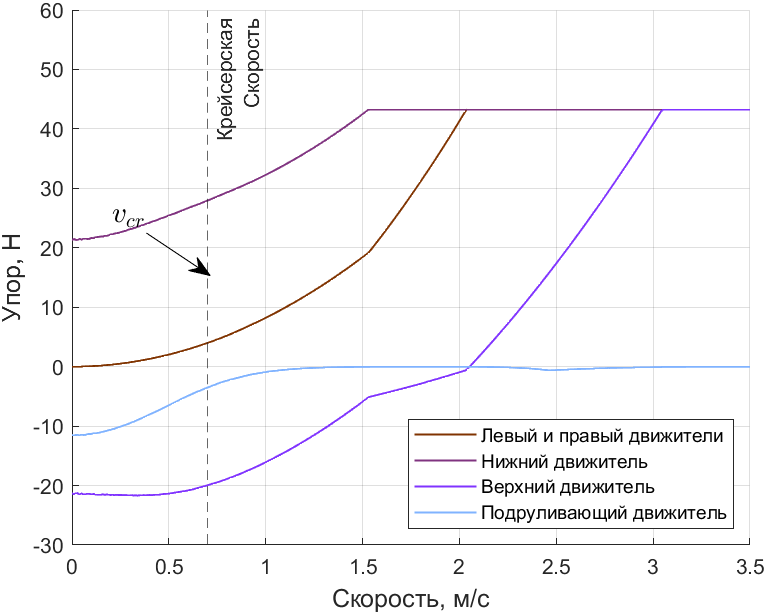
\includegraphics[width=0.5\linewidth]{allocation/Результат ММТ300 - Адаптивный Упоры.png}}
        \hfill
        \subcaptionbox{Сформированные силы и моменты}{%
            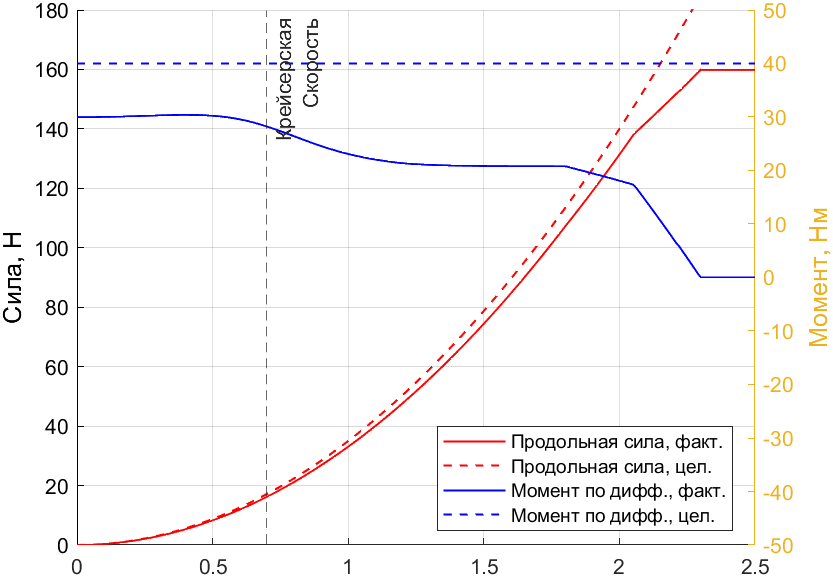
\includegraphics[width=0.5\linewidth]{allocation/Результат ММТ300 - Адаптивный силы.png}}
        \hfill
    }
    \caption*{Рис. 5 -- Распределение упоров и сформированные при этом силы и моменты адаптивным методом управления ДРК.}\label{fig:latex}
\end{figure}

\FloatBarrier
\pdfbookmark{Заключение}{conclusion}                                  % Закладка pdf
В \underline{\textbf{заключении}} приведены основные результаты работы, которые заключаются в следующем:
%% Согласно ГОСТ Р 7.0.11-2011:
%% 5.3.3 В заключении диссертации излагают итоги выполненного исследования, рекомендации, перспективы дальнейшей разработки темы.
%% 9.2.3 В заключении автореферата диссертации излагают итоги данного исследования, рекомендации и перспективы дальнейшей разработки темы.
\begin{enumerate}
  \item Предложен новый метод оценки скорости движения АНПА относительно набегающего потока по изменению параметров работы движителей маршевой группы в установившемся режиме движения. Метод позволяет оценить скорость движения АНПА относительно потока в случае отсутствия основного датчика скорости или выхода его из строя.
  \item Проведена верификация предолженного метода оценки скорости набегающего на обработке данных запусков АНПА ``ММТ-3000''. После уточнения параметров ГВ на калибровочной части маршрута, расхождение оцениваемой скорости с эталонными показаниями доплеровского лага составило не более чем 0.18 м/с на переходных режимах и не более чем 0.1 м/с на установившихся режимах движения со среднеквадратичным отклонением $\sigma=0.17$ м/с.
  \item Предложен новый алгоритм управления ДРК подводного аппарата, который учитывает особенности работы исполнительных механизмов в набегающем потоке и способен адаптивно перераспределять управляющие воздействия при вариациях скорости.
  \item Показано что предложеный метод управления ДРК обеспечивает более высокую скорость работы по сравнению со стандартными подходами к решению задачи управления ДРК через формирование линейной и квадратичной оптимальной задачи при сопосповимой области допустимых значений. По сравнению с используемым в АНПА ``ММТ-300'', предлагаемый метод позволяет обеспечивать более широкий диапазон управления и позволяет удерживать заданный момент при более высоких значениях целевой скорости.
\end{enumerate}


\pdfbookmark{Литература}{bibliography}                                % Закладка pdf

\ifdefmacro{\microtypesetup}{\microtypesetup{protrusion=false}}{} % не рекомендуется применять пакет микротипографики к автоматически генерируемому списку литературы
\urlstyle{rm}                               % ссылки URL обычным шрифтом
\ifnumequal{\value{bibliosel}}{0}{% Встроенная реализация с загрузкой файла через движок bibtex8
    \renewcommand{\bibname}{\large \bibtitleauthor}
    \nocite{*}
    \insertbiblioauthor           % Подключаем Bib-базы
    %\insertbiblioexternal   % !!! bibtex не умеет работать с несколькими библиографиями !!!
}{% Реализация пакетом biblatex через движок biber
    % Цитирования.
    %  * Порядок перечисления определяет порядок в библиографии (только внутри подраздела, если `\insertbiblioauthorgrouped`).
    %  * Если не соблюдать порядок "как для \printbibliography", нумерация в `\insertbiblioauthor` будет кривой.
    %  * Если цитировать каждый источник отдельной командой --- найти некоторые ошибки будет проще.
    %
    %% authorvak

    \ifnumgreater{\value{usefootcite}}{0}{
        \begin{refcontext}[labelprefix={}]
            \ifnum \value{bibgrouped}>0
                \insertbiblioauthorgrouped    % Вывод всех работ автора, сгруппированных по источникам
            \else
                \insertbiblioauthor      % Вывод всех работ автора
            \fi
        \end{refcontext}
    }{
        \ifnum \totvalue{citeexternal}>0
            \begin{refcontext}[labelprefix=A]
                \ifnum \value{bibgrouped}>0
                    \insertbiblioauthorgrouped    % Вывод всех работ автора, сгруппированных по источникам
                \else
                    \insertbiblioauthor      % Вывод всех работ автора
                \fi
            \end{refcontext}
        \else
            \ifnum \value{bibgrouped}>0
                \insertbiblioauthorgrouped    % Вывод всех работ автора, сгруппированных по источникам
            \else
                \insertbiblioauthor      % Вывод всех работ автора
            \fi
        \fi
        %  \insertbiblioauthorimportant  % Вывод наиболее значимых работ автора (определяется в файле characteristic во второй section)
        \begin{refcontext}[labelprefix={}]
            \insertbiblioexternal            % Вывод списка литературы, на которую ссылались в тексте автореферата
        \end{refcontext}
        % Невидимый библиографический список для подсчёта количества внешних публикаций
        % Используется, чтобы убрать приставку "А" у работ автора, если в автореферате нет
        % цитирований внешних источников.
        \printbibliography[heading=nobibheading, section=0, env=countexternal, keyword=biblioexternal, resetnumbers=true]%
    }
}
\ifdefmacro{\microtypesetup}{\microtypesetup{protrusion=true}}{}
\urlstyle{tt}                               % возвращаем установки шрифта ссылок URL
